\documentclass{article}
    \usepackage{caption}
    \usepackage{subcaption}
    \usepackage{mathtools}
    \usepackage{algorithm2e}
    
    \usepackage{enumerate}% section item
    \usepackage{amssymb}  % \varnothing
    \usepackage{booktabs} % insert table
    \usepackage{multirow} % table combine
    \usepackage{listings} % insert code
    \usepackage{appendix} % 
    \usepackage{amsmath}  % for mathfont
    \usepackage{unicode-math} % for mathfont
    \usepackage{fontspec} % set font
    \setmainfont{Times} % main font
    \newfontfamily\monaco{Monaco} % code font
    \usepackage{pythonhighlight} % python
   % \usepackage{hyperref}

    \usepackage{listings}
    \usepackage{color}
    \usepackage{xcolor}
    \definecolor{dkgreen}{rgb}{0,0.6,0}
    \definecolor{gray}{rgb}{0.5,0.5,0.5}
    \definecolor{mauve}{rgb}{0.58,0,0.82}
    \lstset{frame=tb,
        language=Java,
        aboveskip=3mm,
        belowskip=3mm,
        showstringspaces=false,
        columns=flexible,
        basicstyle = \ttfamily\small,
        numbers=none,
        numberstyle=\tiny\color{gray},
        keywordstyle=\color{blue},
        commentstyle=\color{dkgreen},
        stringstyle=\color{mauve},
        breaklines=true,
        breakatwhitespace=true,
        tabsize=3
    }


    \usepackage[colorlinks=true]{hyperref} % the option is there to remove the square around links which is what I don't like.
    
    \usepackage{perpage} 
    \MakePerPage{footnote} % Reset the footnote counter perpage. may require to run latex twice.
    
    \usepackage[margin=2cm]{geometry} % This is here to fit more text into the page.
    
 %   \setcounter{secnumdepth}{1}  % This removes the numbering from the subsections.
                            % If you want the numbering of the subsection level just remove this line
    
    \title{\textsc{COMP7506 - MScApp}}
    \author{	3035562502 - ZHANG Kai \\
                3035562100 - WANG Dezhao \\
                3035562069 - YAN Qiangyu }
    \date{}
    
    \setlength{\parindent}{0pt} % No indentation for paragraphs. Because that is just old.
    \setlength{\parskip}{\baselineskip} % Instead use vertical paragraph spacing.
    
    %\setmainfont{Helvetical} % Setting the main font here. But I like the default font alot so this is commented out.
    
    \begin{document}
    \maketitle
    
    
    \section{Basic framework}

    \begin{center}
        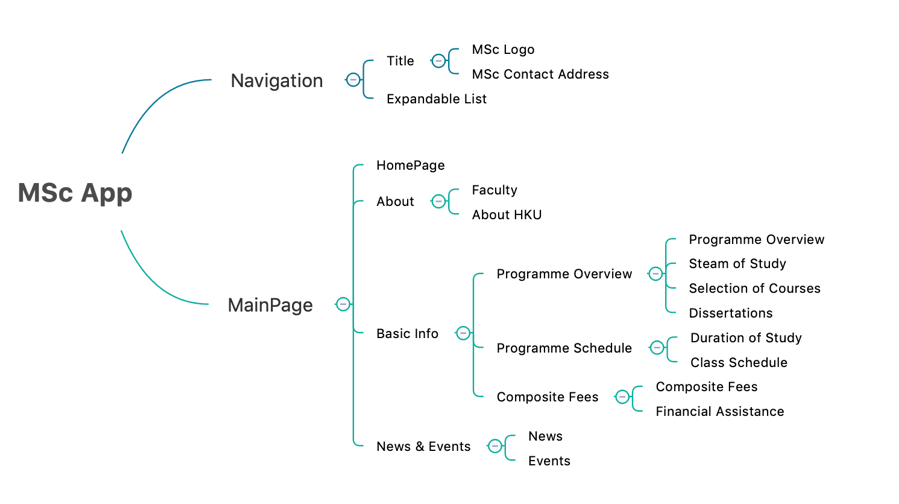
\includegraphics[width=5.5in]{framework}
    \end{center}

    \section{Main functions}

    \begin{enumerate}[a)]
    \item MainActivity.java
    
    The app starts with this activity and 
    set content view to activity\_main.xml.

    \begin{lstlisting}[ language=Java]
private void initNavigationView():
    \end{lstlisting}
    Initialize the menu data in expandableListView and populate the expandable list. Set adapter, setOnGroupClickListener and setOnChildClickListener here.

    \begin{lstlisting}[ language=Java]
private void switchFragment(Fragment targetFragment):
    \end{lstlisting}
Use FragmentManager and FragmentTransaction to switch different fragment.

    \begin{lstlisting}[ language=Java]
public void goBackView()、goForwardView():
    \end{lstlisting}
    Provide an interface to child fragments call to switch views.

    \item ExpandableListAdapter.java
    
    This is customized list adapter extend BaseExpandableListAdapter, 
    we define different function to get child view or group view data here, 
    like :
    \begin{lstlisting}[ language=Java]
public long getChildId(int groupPosition, int childPosition)
public View getChildView(int groupPosition, final int childPosition,
                            boolean isLastChild, View convertView, ViewGroup parent)
public int getChildrenCount(int groupPosition)
public MenuModel getGroup(int groupPosition)
...        
    \end{lstlisting}
    
    \item FragmentHome.java
    
    This is the fragment of homepage implements AppbarLayout.

    \begin{lstlisting}[ language=Java]
private void initToolbar(View view) & initAppBarLayout(View view):
    \end{lstlisting}

    Bind the toggle icon animation with drawer, add drawer listener. 
    And set appbar offsetChangedListener to change alphaScale 
    according to offset height. 

    \begin{lstlisting}[ language=Java]
private void initConvenientBanner(View view):
    \end{lstlisting}

    Use ConvenientBanner and LocalImageHolderView to 
    complete the custom rotation effect with pictures.

    \begin{lstlisting}[ language=Java]
private void initTextViewClick(View view):
    \end{lstlisting}

    Set textView click listener to change fragment view.

    \item LocalImageHolderView.java
    
    A custom HolderView implements Holder.

    \item FragmentAbout.java, FragmentFaculty…FragmentSchedule.java
    
    Different child fragment function, 
    including setting the corresponding view, 
    setting toolbar click listener on icon and 
    initializing view pager with different layout xml files.

    \item LoadingView.java
    A custom loading effect chart and some functions to set its visibility.

    \item FragmentNews.java, FragmentEvents.java
    
    \begin{lstlisting}[ language=Java]
private void initNewThread():
    \end{lstlisting}

    Start new thread and use Jsoup to get information from website. 
    Then parse HTML doc into required elements and 
    generate different Card View.

    \begin{lstlisting}[ language=Java]
getActivity().runOnUiThread(new Runnable() {}):
    \end{lstlisting}

    Update the application UI by using runOnUiThread(). 
    This will magically cause the Runnable code to 
    get executed on the Main Thread.
        
    \end{enumerate}

    \section{Project structure}

    \begin{center}
        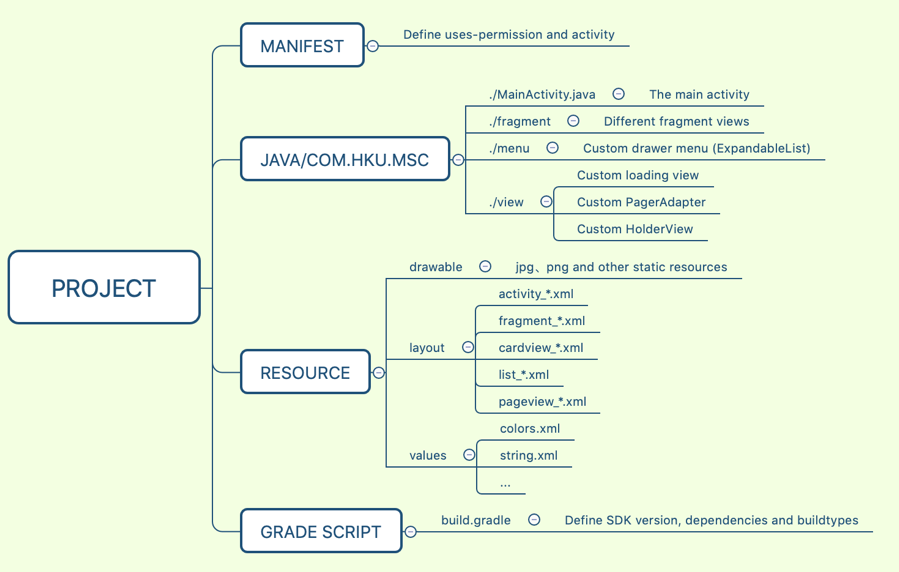
\includegraphics[width=5.5in]{structure}
    \end{center}

    \section{Compilation and Execution process}

    If you want to install the app on your andorid devices, 
    you need to generate the suitable apk. 
    
    Just click Build > Generate Signed APK > app > 
    Create new (sign key) > Next ... > Finish > Reveal the apk in Finder.

    \newpage
    \section{Contributions}

    \begin{table}[h]
        \centering
        \begin{tabular}{|c|l|}
            \hline
            \multirow{7}{*}{ZHANG Kai} &  Main activity with layout/main.xml\\
            \cline{2-2}
            &Switch fragment functions \\
            \cline{2-2}
            &Fragment of homepage, corresponding layout xml file \\
            \cline{2-2}
            &Toolbar function and xml, bind toggle icon with drawer listener \\
            \cline{2-2}
            & Custom HolderView implements Holder, 
            implement automatic scrolling of pictures with\\
            & ConvenientBann\\
            \cline{2-2}
            &Complete the draft documentation, and Readme.md \\
            \hline
            \multirow{7}{*}{WANG Dezhao} &  
            Fragment of basic info (fees, overview, schedule), 
            corresponding layout xml files\\
            \cline{2-2}
            & Fragment of about (faculty, about HKU), 
            corresponding layout xml files \\
            \cline{2-2}
            & Custom ExpandableListAdapter and MenuModel item, 
            with list\_group\_child.xml/ \\
            & list\_group\_header.xml,
             generate custom drawer controls \\
            \cline{2-2}
            & View pager function, custom pager adapter \\
            \cline{2-2}
            & Page view layout files including Programme Overview, 
            Stream of Study, Selection of Courses, \\
            & Dissertations \\
            \hline
            \multirow{7}{*}{YAN Qiangyu} &  
            Fragment of news \& events, corresponding layout xml files\\
            \cline{2-2}
            & Custom loading view \\
            \cline{2-2}
            & Custom card view of news and card view of events \\
            \cline{2-2}
            & Multi-threaded operation when using Jsoup 
            to scratch message from URL and parse HTML \\
            \cline{2-2}
            & Update UI by using UIThread \\
            \cline{2-2}
            & Make the video \\
            \cline{2-2}
            & Review and complete the final documentation \\
            \hline
        \end{tabular}
    \end{table}

    \end{document}